% Preamble
\documentclass[11pt]{article}
\usepackage[letterpaper]{geometry}
\usepackage{cite}
\usepackage{url}
\usepackage{fancyhdr}
% Packages
\usepackage{amsmath}
\usepackage{graphicx}
\usepackage[english]{babel}
\usepackage{lipsum}
\usepackage{wrapfig}
\usepackage[font=small,labelfont=bf]{caption}
\usepackage{xcolor}
\fancypagestyle{firstpage}
{
\fancyhead[L]{}
\fancyhead[R]{Zach Arnold \linebreak CS 7641 \linebreak Assignment 4}
\setlength{\headheight}{52pt}
}
\graphicspath{./}
\newcommand{\problemone}{Small Grid World}
\newcommand{\problemtwo}{Mountain Car}
% Document
\begin{document}
    \thispagestyle{firstpage}


    \section{Introduction}\label{sec:introduction}
    The purpose of this paper is to explore Markov Decision Processes.
    Specifically, analyzing algorithms for solving MDPs in two different problem domains.
    Those domains will have differing characteristics such as state domain, size, and action types in those domains.
    I will attempt to compare the results from three different algorithms, Value Iteration, Policy Iteration, and Q-Learning.


    \section{Problem Descriptions}
    In this section I will talk about the different problems I will be analyzing and why they are interesting.
    \subsection{\problemone}
    This problem is fairly classic in reinforcement learning algorithm analysis.
    The domain of this problem is a 10 x 10 matrix of squares representing a grid which is a subset of the world.
    (See figure~\ref{Fig:Small Grid World} for an example grid world.)
    There are up to 100 unique states in this world and 4 actions that can be taken in any state.
    If we suppose that the grid world were a map with the upward direction being North and the remaining three directions,
    then moving in one of these four directions represent the set of possible actions.
    Associated with each action there are a few parameters I configured:
    \begin{itemize}
        \item Success rate which controls some stochastic actions into the agents actions in the domain. An action taken by the agent will succeed with probability equal to the success rate $\in [0,1]$ and do some other random action otherwise.
        \item Goal reward which controls the reward value of the goal state
        \item Move reward which controls the value for selecting any action and moving to another square on the grid
    \end{itemize}
    Outside of standard walls that bound the outside edge of the grid world I have the option of turning some of the grid
    squares into "walls" themselves in that they cannot be moved into.
    This reduces the total number of states, but can actually make traversing the map harder due to the fact that direct
    routes may not exist.
    I have done this in my grid world problem to exercise the ability of an algorithm (given discount factor) to consider
    other potential paths to the goal state.

    \subsubsection{Why is this problem interesting?}
    This problem is interesting because it exercises many of the core functionalities of the learning and planning algorithms that I am employing.
    Due to its low number of states and actions, as well as its relative simplicity, this problem is compelling in that we should be able to
    quickly derive insights from and still be able to compare to a more complex one.
    Since there is also an element of randomness in the actions taken by an agent, this problem is still reasonably complex
    and requires some form of exploration before directly arriving at an optimal value/policy/Q.
    The introduction of non-traversable squares should exercise the algorithms ability to consider other possible paths
    (even those moving in a direction further from the goal.)

    \subsection{\problemtwo}
    The mountain car problem is also an interesting single agent reinforcement learning MDP problem.
    The problem uses a cosine curve to model a valley and two peaks and the agent needs to find its way via actions to the higher of the two (or the top of the mountain.)
    From the description in the documentation:
    \begin{quote}
        "In this domain you can change the parameters for min/max position and velocity, the scale of the cosine curve on which the car travels, the force of gravity, acceleration, and the amount of time that elapses between simulation/decision steps."\cite{Burlap20}
    \end{quote}
    The actions that an agent can take in this domain are:
    \begin{itemize}
        \item Move Backwards
        \item Move Forwards
        \item Do Nothing
    \end{itemize}
    \subsubsection{Why is this problem interesting?}
    This problem Is interesting given that it has a large number of potential states.
    By large, I mean that it has an infinite number of states given that it is a continuous domain modeled by the cosine curve.
    In order to overcome the requirement by value iteration and policy iteration in BURLAP to be able to determine all
    states that are reachable I will be sampling 5000 states from a uniform distribution positions along this curve.
    Whereas in the grid world there was some stochastic randomness to the transition function between states, the agent
    in this world will have different external forces to overcome, namely the force of gravity and the lack of friction
    whereby an agent could perform no actions and still experience a transition (othwerwise known as momentum.)
    Given all these it will be interesting to see the results of the algorithms on this problem.


    \section{Algorithms}
    In this section we will talk about the algorithms I will be using to analyze these problems as well as the parameters
    that I will vary in search of an optimal solution to these problems.
    \subsection{Parameter Exploration}
    \begin{itemize}
        \item $\gamma$ which is the discount factor where $\gamma \in [0,1]$ and manages the explore/exploit dilemma in RL where high values favor long-term rewards, and low values optimize for greedier short-term rewards
        \item $\delta$ which controls the threshold that if Policy Iteration, Value Iteration, or Q-Learning improve by less than this value, then the algorithm terminates
        \item Initial Q Value initialized optimitically in my case of 0.3
        \item $\alpha$ which controls the learning rate of the respective algorithms
        \item Number of Trials, which dictates the number of times to re-run a learning session with a particular algorithm, the average reward of which is taken as the final result
    \end{itemize}
    \subsection{Value Iteration}
    For both problems I used the BURLAP implementation of value iteration to derive the optimal reward values for each state
    according to the Bellman update rule.
    Even though Value Iteration is guaranteed to converge, in order to keep my experiments from taking forever, I leveraged
    from the params above to terminate the updates after a threshold or maxiumum iterations occurs.
    \subsection{Policy Iteration}
    \subsection{Q-Learning}



    \section{Analysis}

    \begin{figure}
        \begin{minipage}{0.5\textwidth}
            \centering
            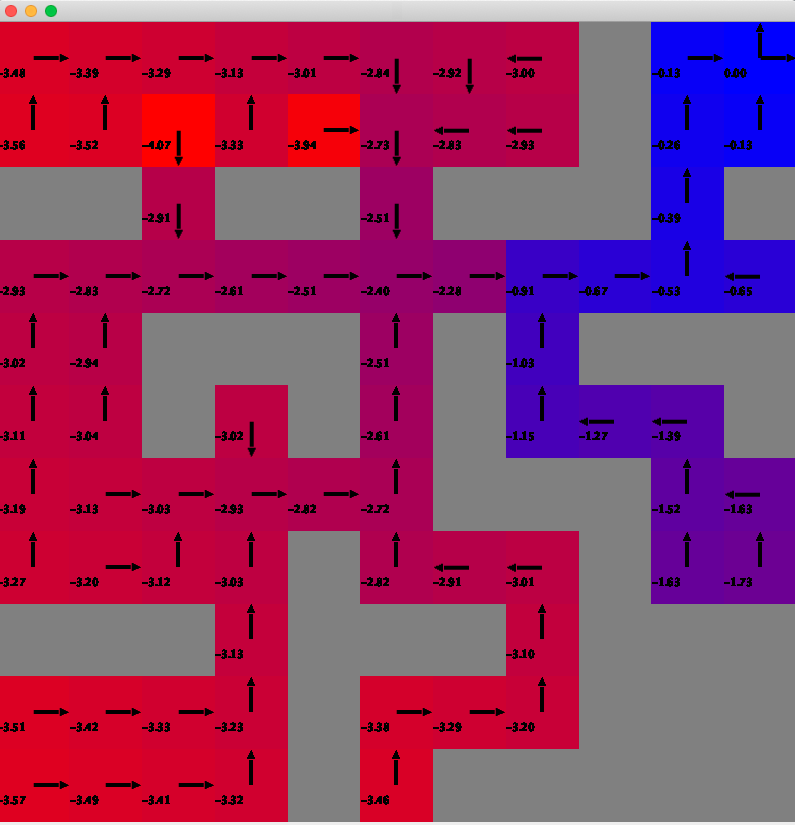
\includegraphics[width=1\linewidth]{smallgridworld.png}
            \caption{Small Grid World}\label{Fig:Small Grid World}
        \end{minipage}
        \begin{minipage}{0.5\textwidth}
            \centering
            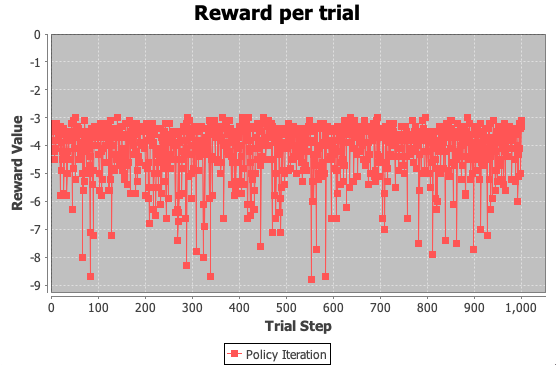
\includegraphics[width=0.99\linewidth]{policyiterationreward.png}
            \caption{Policy Iteration \problemone}\label{Fig:Policy Iteration \problemone}
        \end{minipage}
    \end{figure}

    \begin{figure}
        \begin{minipage}{0.5\textwidth}
            \centering
            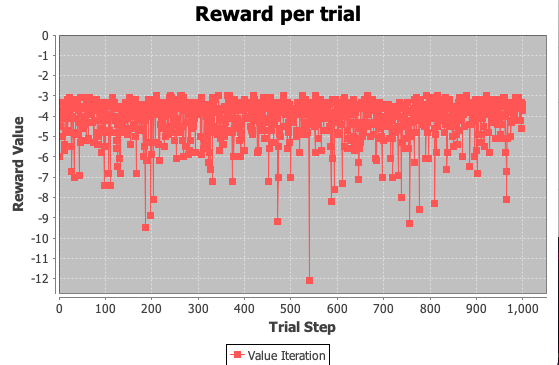
\includegraphics[width=1\linewidth]{valueiterationreward.png}
            \caption{Value Iteration \problemone}\label{Fig:Value Iteration \problemone}
        \end{minipage}
        \begin{minipage}{0.5\textwidth}
            \centering
            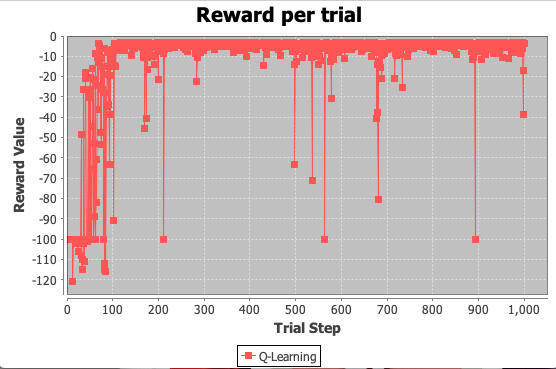
\includegraphics[width=1\linewidth]{qlearningreward.png}
            \caption{Q-Learning \problemone}\label{Fig:Q-Learning \problemone}
        \end{minipage}
    \end{figure}
    \begin{figure}
        \begin{minipage}{1\textwidth}
            \centering
            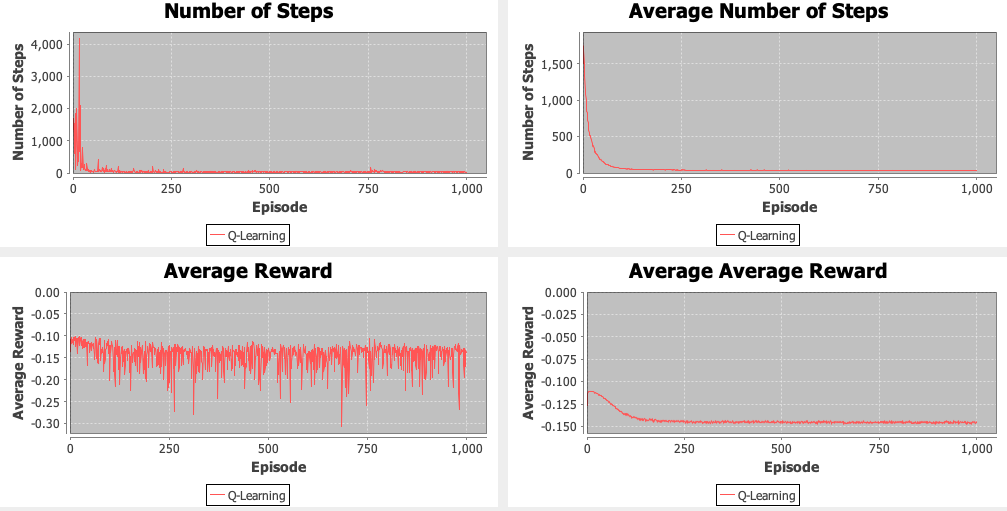
\includegraphics[width=1\linewidth]{qlearningdeepdive.png}
            \caption{Q Learning Analysis \problemone}\label{Fig:Q-Learning DD \problemone}
        \end{minipage}
    \end{figure}
    \section{Conclusion}
    In this paper I have explored the tradeoffs between algorithms
    \bibliography{bibliography}
    \bibliographystyle{plain}
\end{document}